\documentclass[aspectratio=169]{beamer}

%includeonlyframes{current}

\usepackage[T1]{fontenc}
\usepackage[utf8]{inputenc}
\usepackage[american]{babel}
\usepackage{amsmath,amsthm}
\usepackage{multirow}
\usepackage{tikz}
\usetikzlibrary{matrix,decorations,decorations.text,calc,arrows,snakes,shapes,positioning}
\usepackage{multimedia}

\usepackage[nosfdefault]{comicneue}
\usepackage{sourcesanspro}
\usepackage[amssymb,amsfonts]{concmath}
\usefonttheme[onlymath]{serif}
\usepackage{ulem}

\mode<presentation>{%
  \usetheme{ibm}
}

\newcommand{\F}{\mathbb{F}}
\newcommand{\Z}{\mathbb{Z}}
\newcommand{\Q}{\mathbb{Q}}
\DeclareMathOperator{\End}{End}
\DeclareMathOperator{\Cl}{Cl}
\DeclareMathOperator{\poly}{poly}
\DeclareMathOperator{\polylog}{polylog}

../share/isographs.tex

\title[VDFs from Supersingular Isogenies and Pairings]{Verifiable Delay Functions from Supersingular Isogenies and Pairings}
\author[Luca De Feo]{
  Luca De Feo\\[1em]
  based on joint work with J.~Burdges, S.~Masson, C.~Petit, A.~Sanso}
\date{November 12, 2020, CV Labs}
\institute{IBM Research Zürich}

\begin{document}

\frame[plain]{\titlepage}

%% 

\begin{frame}{Computational hardness in cryptography}
  \begin{center}
    \framebox{\textcolor{gray}{boring picture of Alice, Bob and Eve goes here}}
  \end{center}

  \medskip
  
  \textbf{\emph{How long} will it take Eve to decrypt the message?}
  \smallskip
  \begin{description}
  \item[Complexity theory:] (sub)exponentially more than Bob.
    \begin{itemize}
    \item Asymptotics don't say anything on constants.
    \item Based on an \emph{average-case} analysis, ignores
      \emph{worst case}.
    \item Typically based on a Turing-machine or RAM-like model,
      doesn't necessarily fit reality.
    \end{itemize}
  \item[Real world crypto:] at least $2^{128}$ ``operations''.
    \begin{itemize}
    \item But what's an ``operation''?
    \item Often based on extrapolations (see, in particular, factoring).
    \item Doesn't account for parallelism.
    \item More a measure of \emph{cost} than a measure of \emph{time}.
    \end{itemize}
  \end{description}
\end{frame}

%%

\begin{frame}{Time-lock Puzzles}
  \begin{center}
    \begin{tikzpicture}
      \node (fred) at (0,0) {\includegraphics[height=6em]{fred.png}};
      \node (jets) at (9.2,0) {\includegraphics[height=7em]{jetsons.png}};
      
      \foreach \i in {2,...,6} {
        \pgfmathparse{int(14-2*\i)}
        \let\time\pgfmathresult
        \uncover<\i>{
          \draw (\i,0.5) node {\includegraphics[width=2em]{chest-closed.png}};
          \draw (4.6,-0.5) node {\comicneue\bfseries\footnotesize OPEN IN \time 00000 YEARS};
          \draw[thick,->] (fred) edge (\i+1,0);
        }
      }
      \uncover<7>{
        \draw (7,0.5) node {\includegraphics[width=2em]{chest-open.png}};
        \draw (4.6,-0.5) node {\comicneue\bfseries\footnotesize YABBA DABBA DOO!};
        \draw[thick,->] (fred) edge (8,0);
      }
    \end{tikzpicture}
  \end{center}

  Basically a \emph{Key Derivation Function} (family) with two
  algorithms: \medskip
  \begin{description}
  \item[KDF$(T, \Delta)$:] which computes a \emph{key} $k$
    given a \emph{trapdoor} $T$ and a \emph{delay} $\Delta$.
  \item[SlowKDF$(\Delta)$:] which computes the same key $k$
    without knowledge of the trapdoor,\\
    \emph{in time approximately $\Delta\cdot\mathrm{constant}$}.
  \end{description}
  \smallskip \dots under the conjecture that no algorithm faster than
  SlowKDF can compute $k$ from $\Delta$ with non-negligible
  probability.
\end{frame}

%%

\begin{frame}{Some applications}
  \begin{block}{Sealed bid auctions}
    Standard solution based on encryption:
    \begin{itemize}
    \item Each bidder encrypts its bid;
    \item At the end of the auction each bidder reveals the key.
    \end{itemize}

    \emph{Problem:} some bidders may refuse to reveal the key.\\
    \textcolor{gray}{Especially important in Vickrey auctions (winner
      pays second highest bid).}

    \bigskip\pause
    Solution:
    \begin{itemize}
    \item Each bidder encrypts bid with a TL puzzle;
    \item At the end of the auction each well behaved bidder reveals
      its trapdoor;
    \item Other bids are opened with SlowKDF. \textcolor{gray}{(can
        get quite expensive, though)}
    \end{itemize}
    
    \smallskip\pause More efficient solution provided by
    \emph{Homomorphic TL} or \emph{Delay Encryption}: not this talk.
  \end{block}

  \pause
  Other applications: Voting, key escrow, \dots
\end{frame}

%%

\begin{frame}{Verifiable Delay Functions (Boneh, Bonneau, Bünz, Fisch 2018)}
  \begin{columns}
    \begin{column}{0.2\textwidth}
      \centering
      \includegraphics[width=0.8\textwidth]{phileas_fogg}

      \vfill

      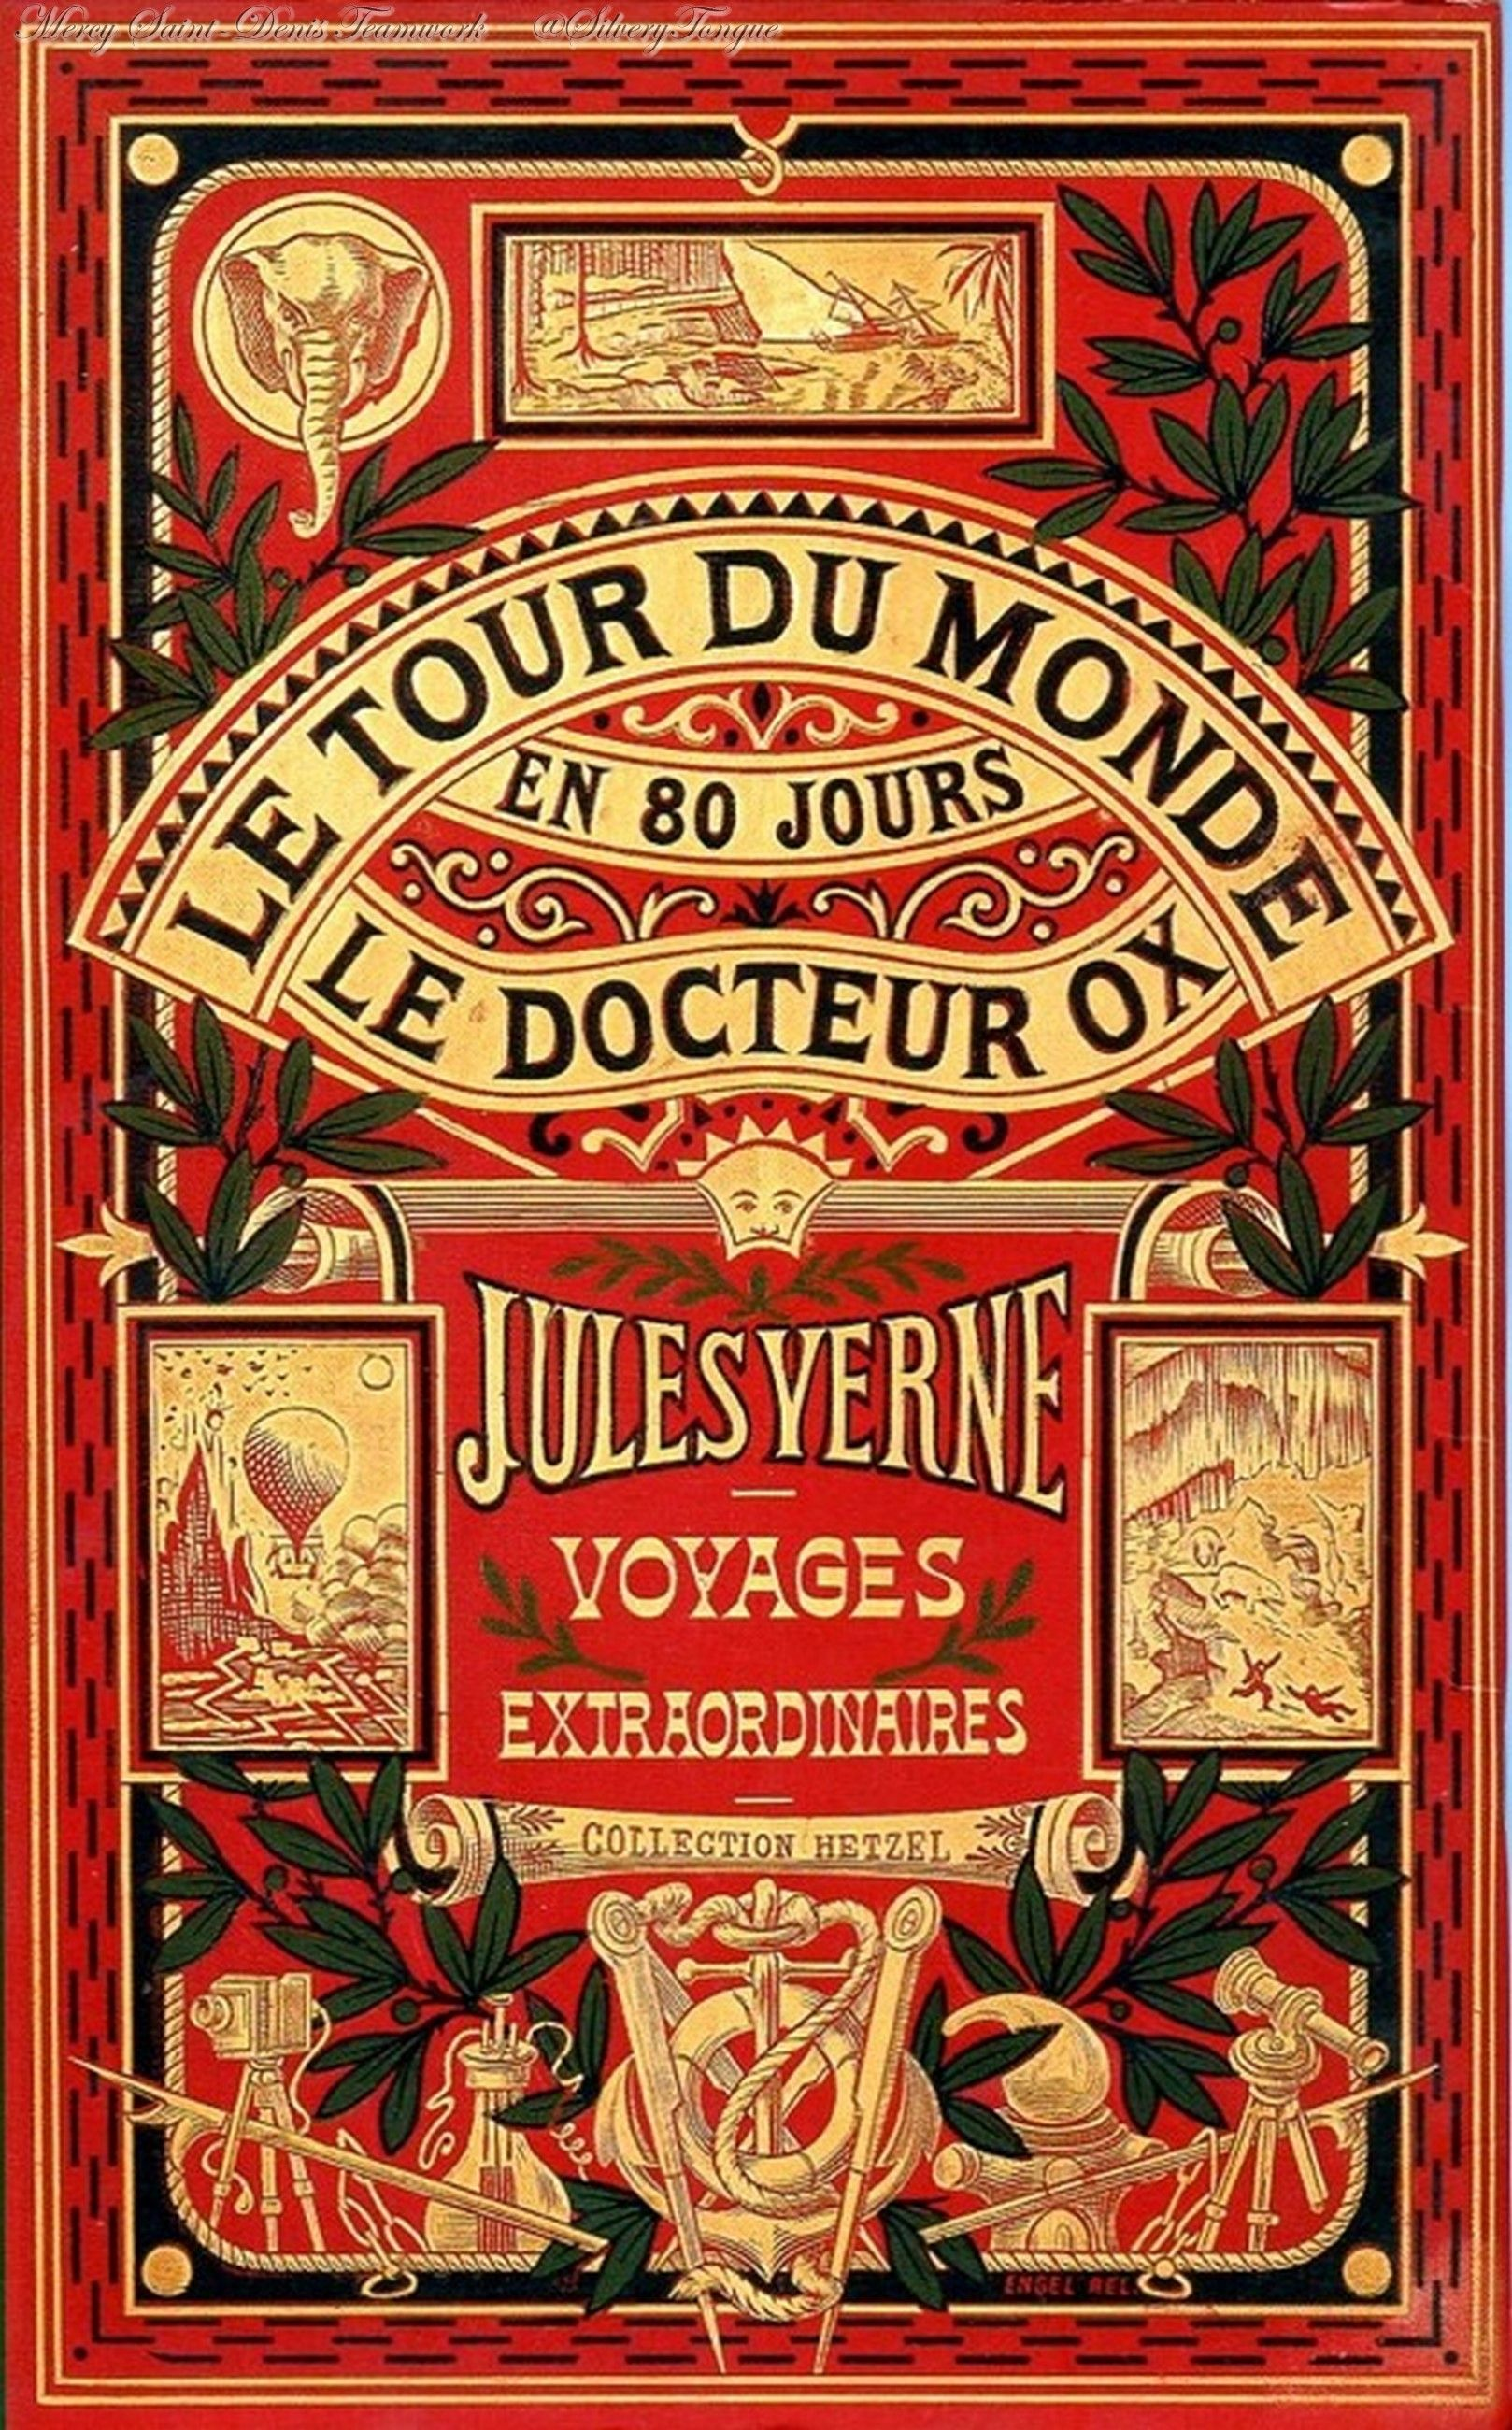
\includegraphics[width=0.8\textwidth]{80jours-couverture}
    \end{column}
    \begin{column}{0.75\textwidth}
      \begin{block}{A sort of \textit{deterministic Proof of Sequential Work}}
        Function (family) \emph{$f:X\to Y$} s.t.:

        \begin{itemize}
        \item Evaluating $f(x)$ takes \emph{long time}:
          \begin{itemize}
          \item \emph{predictably} long time,
          \item on almost all random inputs $x$,
          \item even after having seen many values $f(x')$,
          \item even given \emph{massive number of processors};
          \end{itemize}
        \item Verifying $y=f(x)$ is \emph{efficient}:
          \begin{itemize}
          \item ideally, exponential separation between evaluation and
            verification.
          \end{itemize}
        \end{itemize}
      \end{block}
    \end{column}
  \end{columns}
\end{frame}

%%

\begin{frame}{Example: distributed lotteries}
  Participants \textbf{A, B, \dots, Z} want to agree on a random
  winning ticket.

  \begin{block}{Flawed protocol}
    \begin{itemize}
    \item Each participant \emph{$x$} broadcasts a random string
      \emph{$s_x$};
    \item Winning ticket is \emph{$H(s_A, \dots, s_Z)$}.
    \end{itemize}

    \pause
    
    Cheating participant \textbf{Z} waits to see all other strings,
    then brute-forces \emph{$s_Z$} to win lottery.
  \end{block}
  
  \pause

  \begin{block}{Fixes}
    \begin{itemize}
    \item Make the hash function \textbf{sloooooooooooooooooooooooooooow};
      \begin{itemize}
      \item e.g., participants have 10 minutes to submit $s_x$,
      \item outcome will be known after 20 minutes.
      \end{itemize}
    \item<4-> Make it possible to verify \emph{$w = H(s_A, \dots, s_Z)$} \textbf{fast}.
    \end{itemize}
  \end{block}
\end{frame}

%%

\begin{frame}{Applications}
  \begin{block}{Randomness beacons}
    \begin{description}
    \item[Goal:] Generate a public stream of provably random numbers.
    \item[Standard technique:] Hash output of public high entropy
      sources (e.g.: stock market, weather, \dots) at regular
      intervals (epochs).
    \item[Risk:] Close to the end of the epoch, adversary manipulates
      the data (e.g., buys stock) repeatedly until they get the
      desired alea.
    \item[Fix:] Run the hashed value through a VDF with delay longer
      than the epoch.
    \end{description}
  \end{block}

  \begin{block}{Proofs of Stake/Space}
    \begin{description}
    \item[Goal:] Elect epoch leader(s) in PoS blockchains.
    \item[Standard technique:] PoS are assigned a ``quality'' (e.g.:
      hash of the PoS), the higher quality gets elected as leader.
    \item[Disadvantage:] Requires synchronization of miners.
    \item[Fix (Chia):] Run the PoS through a VDF with delay
      proportional to quality.
    \end{description}
  \end{block}
\end{frame}

%%

\begin{frame}{VDF Craze}
  Who is investing in VDFs

  \begin{description}
  \item[VDF Alliance\footnote{\url{https://www.vdfalliance.org/}}:]
    formed by Etherereum, Protocol Labs, Tezos, Interchain,
    Supranational.
  \item[VDF competitions] (cash prizes in the order of 100k\$):
    \begin{itemize}
    \item RSA-based, run by VDF
      Alliance\footnote{\url{https://supranational.atlassian.net/wiki/spaces/VA/pages/36569208/FPGA+Competition}}.
      \begin{itemize}
      \item Squaring modulo $N$,
      \item Distributed generation of RSA numbers.
      \end{itemize}
    \item Class group based, run by
      Chia\footnote{\url{https://github.com/Chia-Network/vdf-competition/}}.
      \begin{itemize}
      \item Class number computation.
      \item Squaring in class groups.
      \end{itemize}
    \end{itemize}
  \item[More resources:] \url{https://vdfresearch.org/}.
  \end{description}
\end{frame}

%%

\begin{frame}[plain]
  \begin{beamercolorbox}[sep=0.1px,center,wd=\paperwidth,ht=\paperheight]{palette tertiary}
    \begin{columns}
      \begin{column}{0.55\textwidth}
        \Huge\centering Group based\\Delay Functions
      \end{column}
      \begin{column}{0.45\textwidth}
        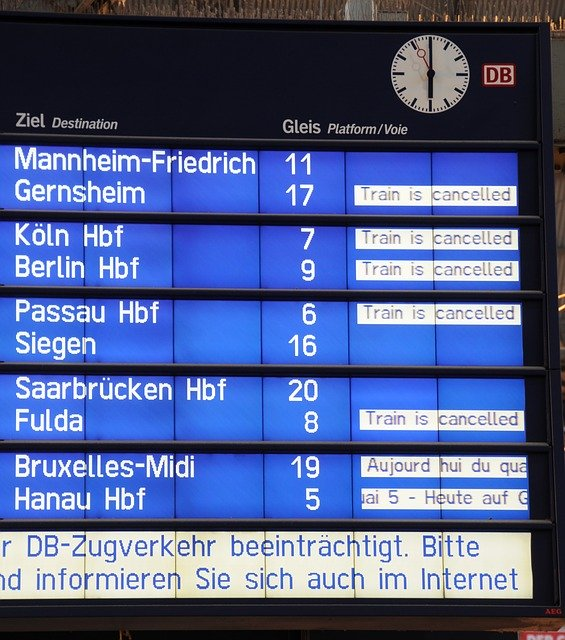
\includegraphics[height=\paperheight]{db.jpg}
      \end{column}
    \end{columns}
  \end{beamercolorbox}
\end{frame}

%%

\begin{frame}[label=current]{Rivest-Shamir-Wagner TL Puzzle ('96)}
  \begin{columns}
    \begin{column}{0.6\textwidth}
      \begin{block}{Setup}
        \emph{$\Z/N\Z$} with $N=pq$ an RSA modulus\\
        $N$ \emph{public}, $p,q$ \emph{private}
      \end{block}

      \begin{block}{Slow KDF}
        With \emph{delay parameter} $\Delta$:
        \begin{align*}
          f:(\Z/N\Z)^\times &\longrightarrow (\Z/N\Z)^\times\\
          x &\longmapsto x^{2^\Delta}
        \end{align*}
        (Conjecturally) takes $\Delta$ squarings.
      \end{block}
    \end{column}
    \begin{column}{0.37\textwidth}
      \centering
      \begin{tikzpicture}[x=2cm,y=2cm]
        \def\crater{29}
        \draw[fill] (360/\crater:1) circle (1pt) +(360/\crater:1em) node {$x$};
        \uncover<2->{
          \draw[fill] (360/\crater : 1) -- (360/\crater*2 : 1)
          circle (1pt) +(360/\crater*2:1em) node {$x^2$};
        }
        \uncover<3->{
          \draw[fill] (360/\crater*2 : 1) -- (360/\crater*3 : 1)
          circle (1pt) +(360/\crater*3:1em) node {$x^4$};
        }
        \uncover<4->{
          \draw[dotted] (360/\crater*3 : 1) arc (360/\crater*3:360/\crater*23:1);
          \draw[fill] (360/\crater*23 : 1) circle (1pt) +(360/\crater*23:1em) node {$x^{2^\Delta}$};
        }
        \uncover<5->{
          \draw[red] (360/\crater : 1) -- node[auto] {$2^\Delta\bmod \varphi(N)$} (360/\crater*23 : 1);
        }
      \end{tikzpicture}

      \medskip
      \uncover<5->{
        \emph{KDF:} knowing $p,q$, we can take a shortcut!
      }
    \end{column}
  \end{columns}
\end{frame}

%%

\begin{frame}[label=current]{VDFs from groups of unknown order}
  \transdissolve<1>
  \begin{columns}
    \begin{column}{0.6\textwidth}
      \begin{block}{Setup}
        \emph{$\Z/N\Z$} with $N=pq$ an RSA modulus,\\
        $N$ \emph{public}, $p,q$ \emph{unknown}
      \end{block}

      \begin{block}{Evaluation}
        With \emph{delay parameter} $\Delta$:
        \begin{align*}
          f:(\Z/N\Z)^\times &\longrightarrow (\Z/N\Z)^\times\\
          x &\longmapsto x^{2^\Delta}
        \end{align*}
        (Conjecturally) takes $\Delta$ squarings.
      \end{block}
    \end{column}
    \begin{column}{0.37\textwidth}
      \centering
      \begin{tikzpicture}[x=2cm,y=2cm]
        \def\crater{29}
        \draw[fill] (360/\crater:1) circle (1pt) +(360/\crater:1em) node {$x$};
        \draw[fill] (360/\crater : 1) -- (360/\crater*2 : 1)
        circle (1pt) +(360/\crater*2:1em) node {$x^2$};
        \draw[fill] (360/\crater*2 : 1) -- (360/\crater*3 : 1)
        circle (1pt) +(360/\crater*3:1em) node {$x^4$};
        \draw[dotted] (360/\crater*3 : 1) arc (360/\crater*3:360/\crater*23:1);
        \draw[fill] (360/\crater*23 : 1) circle (1pt) +(360/\crater*23:1em) node {$x^{2^\Delta}$};
        \draw[red] (360/\crater : 1) -- node[auto] {$2^\Delta\bmod \varphi(N)$} (360/\crater*23 : 1);
      \end{tikzpicture}

      \medskip
      \uncover<2->{
        If we knew $p,q$, then we could easily verify\dots
      }
      \uncover<3->{
        but we don't!
      }
    \end{column}
  \end{columns}
\end{frame}

%%

\begin{frame}[label=current]{VDFs from groups of unknown order}
  \begin{block}{Proofs of exponentiation}
    \begin{description}
    \item[Pietrzak:] recursive argument, rather expensive, low order
      assumption.
   \item[Wesolowski:] arithmetic argument, cheaper, \textit{ad hoc}
      assumption.
    \end{description}
    
    Both made non-interactive via the Fiat-Shamir transform.
  \end{block}

  \pause
  
  \begin{block}{Removing trusted third parties}
    \begin{itemize}
    \item RSA setup requires \emph{trusted generation of $N=pq$}
      (single or distributed authority);
    \item The only property used by the VDFs is that \emph{the order
        of $(\Z/N\Z)^\times$ is unknown};
    \item Can adapt the protocol to any cryptographic \emph{group of
        unknown order}:
      \begin{itemize}
      \item e.g., \emph{quadratic imaginary class groups} of unknown
        order can be publicly generated with no trusted setup!
      \end{itemize}
    \end{itemize}
  \end{block}
\end{frame}

%%

\begin{frame}{The passage of time}
  Some (problematic?) key assumptions:
  \begin{itemize}
  \item A squaring is a squaring. It cannot possibly go faster than \emph{xxx ns}!
  \item You have a machine that computes a squaring in not much
    more than that!
  \item \emph{$n$ squarings} are $n$ squarings. It cannot take less
    than \emph{$n \times $ one squaring} to do them!
  \item Crucially, even if you have $n$ \emph{parallel processors}!
  \end{itemize}
  These are likely all false, but seem to hold in practice\dots
  
  \medskip\pause

  Some concrete numbers:
  \begin{itemize}
  \item 1 squaring modulo a 2048-bits integer (unknown factorization)
    \begin{itemize}
    \item takes \emph{$\approx 1\mu$s in software};
    \item the current record in \emph{FPGA is 25ns}.
    \end{itemize}
  \item Some example delays:
    \begin{itemize}
    \item 1 hour $\qquad\rightarrow\quad\approx 2^{38}$ squarings,
    \item 1 year $\qquad\rightarrow\quad\approx 2^{51}$ squarings,
    \item 1M years $\quad\rightarrow\quad\approx 2^{71}$ squarings.
    \end{itemize}
  \end{itemize}
\end{frame}

%%

\begin{frame}[plain]
  \begin{beamercolorbox}[sep=0.1px,center,wd=\paperwidth,ht=\paperheight]{palette tertiary}
    \begin{columns}
      \begin{column}{0.64\textwidth}
        \Huge\centering Isogeny based\\Delay Functions
      \end{column}
      \begin{column}{0.36\textwidth}
        \includegraphics[height=\paperheight]{phileas_fogg.jpg}
      \end{column}
    \end{columns}
  \end{beamercolorbox}
\end{frame}

%%

\begin{frame}{Elliptic curves and isogenies}
  \begin{columns}
    \begin{column}{0.4\textwidth}
      Elliptic curves
      
      \[y^2 = x^3 + ax + b\]
      
      and their famous \emph{group law}\dots

      \bigskip
      
      \uncover<2->{Isogenies are \emph{morphisms} of elliptic curves.}

      \bigskip
      
      \uncover<3->{\[\frac{\text{Elliptic curves}}{\text{Isogenies}} =
          \frac{\text{Vector spaces}}{\text{Matrices}}\]}
    \end{column}
    \begin{column}{0.6\textwidth}
      \begin{center}
        \begin{tikzpicture}[domain=-2.4566:4,samples=100,yscale=1/2]
          \draw plot (\x,{sqrt(\x*\x*\x-4*\x+5)});
          \draw plot (\x,{-sqrt(\x*\x*\x-4*\x+5)});

          \draw[thin,gray,-latex] (0,-7) -- (0,7);
          \draw[thin,gray,-latex] (-3,0) -- (4,0);
          \draw (-3,1) -- (4,8/3+3);
          \begin{scope}[every node/.style={draw,circle,inner sep=1pt,fill},cm={1,2/3,0,0,(0,3)}]
            \node at (-2.287980,0) {};
            \node at (-0.535051,0) {};
            \node at (3.267475,0) {};
          \end{scope}
          \begin{scope}[every node/.style={yshift=0.3cm},cm={1,2/3,0,0,(0,3)}]
            \node at (-2.287980,0) {$P$};
            \node at (-0.535051,0) {$Q$};
            \node at (3.267475,0) {$R$};
          \end{scope}

          \draw[dashed] (3.267475,3.267475*2/3+3) -- (3.267475,-3.267475*2/3-3) 
          node[draw,circle,inner sep=1pt,fill] {}
          node[xshift=-0.1cm,anchor=east] {$P+Q$};
        \end{tikzpicture}
      \end{center}
    \end{column}
  \end{columns}
\end{frame}

%%

\begin{frame}{Isogenies: an example over $\F_{11}$}
  \centering
  \begin{tikzpicture}[scale=0.4]
    \begin{scope}
      \node[anchor=center] at (0,7) {$E \;:\; y^2 = x^3 + x$};

      \uncover<-1>{
        \draw[thin,gray] (0,-6) -- (0,6);
        \draw[thin,gray] (-6,0) -- (6,0);
      }

      \foreach \x/\y in {0/0,5/3,-4/3,-3/5,-2/1,-1/3} {
        \draw[blue,fill] (\x,\y) circle (0.2) node(E_\x_\y){}
        (\x,-\y) circle (0.2) node(E_\x_-\y){};
      }

      \uncover<2->{\draw[red,fill] (0,0) circle (0.3);}
    \end{scope}

    \draw[black!10!white,thick] (10,-7) -- +(0,14);
    
    \begin{scope}[shift={(20,0)}]
      \node at (0,7) {$E' \;:\; y^2 = x^3 - 4x$};

      \uncover<-1>{
        \draw[thin,gray] (0,-6) -- (0,6);
        \draw[thin,gray] (-6,0) -- (6,0);
      }

      \foreach \x/\y in {0/0,2/0,3/2,4/2,6/4,-2/0,-1/5} {
        \draw[color=blue,fill] (\x,\y) circle (0.2) node(F_\x_\y){}
        (\x,-\y) circle (0.2) node(F_\x_-\y){};
      }
    \end{scope}

    \begin{scope}[color=red,-latex,dashed]
      \begin{uncoverenv}<2->
        \path
        (E_5_3) edge (F_3_2)
        (E_-4_3) edge (F_4_-2)
        (E_-3_5) edge (F_4_2)
        (E_-2_1) edge (F_3_-2)
        (E_-1_3) edge (F_-2_0);
      \end{uncoverenv}
      \begin{uncoverenv}<2->
        \path
        (E_5_-3) edge (F_3_-2)
        (E_-4_-3) edge (F_4_2)
        (E_-3_-5) edge (F_4_-2)
        (E_-2_-1) edge (F_3_2)
        (E_-1_-3) edge (F_-2_0);
      \end{uncoverenv}
    \end{scope}
  \end{tikzpicture}
  
  \begin{columns}
    \begin{column}{0.5\textwidth}
      \[\phi(x,y) = \left(\frac{x^2 + 1}{x},\quad y\frac{x^2-1}{x^2}\right)\]
    \end{column}
    \begin{column}{0.5\textwidth}
      \begin{itemize}
      \item<2-> Kernel generator in \alert{red}.
      \item<2-> This is a degree $2$ map.
      \item<2-> Analogous to $x\mapsto x^2$ in $\F_q^*$.
      \end{itemize}
    \end{column}
  \end{columns}
\end{frame}

%%

\begin{frame}{Up to \emph{isomorphism}}
  \begin{center}
    \begin{tikzpicture}[domain=-2.4566:4,samples=100]
      \newcount\zoomout
      \transduration<15-21>{0.5}
      \animatevalue<15-20>{\zoomout}{0}{10}
      \begin{uncoverenv}<-20>
        \begin{scope}[scale=1-0.09*\zoomout]
          \begin{scope}
            \draw[thin,gray,-latex] (0,-4) -- (0,4);
            \draw[thin,gray,-latex] (-4.2,0) -- (7,0);
          \end{scope}
          
          \newcount\xstretch
          \newcount\ystretch
          \newcount\slant
          \transduration<1-13>{0.5}
          \animatevalue<1-5>{\xstretch}{0}{4}
          \animatevalue<5-9>{\ystretch}{0}{4}
          \animatevalue<9-13>{\slant}{0}{4}      
          \begin{scope}[yscale=0.55-0.05*\the\ystretch,xscale=1+0.1*\the\xstretch,xslant=0.02*\slant]
            \draw plot (\x,{sqrt(\x*\x*\x-4*\x+5)});
            \draw plot (\x,{-sqrt(\x*\x*\x-4*\x+5)});

            \begin{uncoverenv}<-18>
              \draw (-3,1) -- (4,8/3+3);
              \begin{scope}[every node/.style={draw,circle,inner sep=1pt,fill},cm={1,2/3,0,0,(0,3)}]
                \node at (-2.287980,0) {};
                \node at (-0.535051,0) {};
                \node at (3.267475,0) {};
              \end{scope}
              \begin{scope}[every node/.style={yshift=0.3cm},cm={1,2/3,0,0,(0,3)}]
                \node at (-2.287980,0) {$P$};
                \node at (-0.535051,0) {$Q$};
                \node at (3.267475,0) {$R$};
              \end{scope}
              \draw[dashed] (3.267475,3.267475*2/3+3) -- (3.267475,-3.267475*2/3-3) 
              node[draw,circle,inner sep=1pt,fill] {}
              node[xshift=-0.1cm,anchor=east] {$P+Q$};
            \end{uncoverenv}
          \end{scope}

          \begin{uncoverenv}<14>
            \node[anchor=west] at (-4,-3) {\Large\alert{$y^2=x^3+ax+b \quad\longrightarrow\quad j\equiv 1728\frac{4a^3}{4a^3+27b^2}$}};
          \end{uncoverenv}
        \end{scope}
      \end{uncoverenv}
      
      \begin{uncoverenv}<21->
        \draw[fill] (0,0) circle (2pt) node[anchor=north] {$j=1728$};
        \uncover<22>{
          \draw (0.1,0) edge[bend left,->] node[auto] {$\phi$} (7,0);
        }
        \uncover<22->{
          \draw[fill] (7.1,0) circle (2pt) node[anchor=north] {$j=287496$};
        }
        \uncover<23->{
          \draw (0.1,0) edge[bend left,<->,red,very thick] (7,0);
        }
      \end{uncoverenv}
    \end{tikzpicture}
  \end{center}  
\end{frame}

%%

\begin{frame}{The beauty and the beast {\quad\footnotesize(credit: Lorenz Panny)}}
  \begin{overlayarea}{\textwidth}{\textheight}
    \smallskip
    \begin{center}

      Components of particular isogeny graphs look like this:
      \par\vspace{1ex}

      \begin{minipage}{.49\textwidth}\centering
        \begin{tikzpicture}[scale=.6,>=stealth,shorten >=.2mm,shorten <=.2mm,rotate=90,line width=.6pt]
          \isoggraph
        \end{tikzpicture}
      \end{minipage}
      % 
      \begin{minipage}{.49\textwidth}\centering
        \begin{tikzpicture}[scale=2.456,>=stealth,shorten >=.2mm,shorten <=.2mm,rotate=90,line width=.6pt]
          \fpsqgraph
        \end{tikzpicture}
      \end{minipage}

      \only<-2>{
        \vspace{3ex}

        \textit{Which of these is good for VDFs?}
        \pause
        \onslide<2>{%
          \,\textbf{Both!}
        }
      }

    \end{center}
  \end{overlayarea}
\end{frame}

%%

\begin{frame}{Slooooooooooooooooooooooow isogenies (\url{https://ia.cr/2019/166})}
  \begin{columns}
    \begin{column}{0.6\textwidth}
      \begin{block}{Setup}
        With \emph{delay parameter} $T$:
        \begin{itemize}
        \item A looooooooooooooooooooooooong isogeny path,
        \item<2-> A \emph{starting curve} $E_0$,
        \item<2-> An isogeny \emph{$\phi:E_0\to E_T$} of degree \emph{$2^T$}.
        \end{itemize}
      \end{block}

      \begin{uncoverenv}<3->
        \begin{block}{Evaluation}
          $\phi$ \textbf{is} the VDF:
          \begin{align*}
            \phi:E_0(\F_p) &\longrightarrow E_T(\F_p)\\
            P &\longmapsto \phi(P)
          \end{align*}
          Conjecturally, no faster way than \emph{composing degree $2$
            isogenies}.
        \end{block}
      \end{uncoverenv}
    \end{column}
    \begin{column}{0.37\textwidth}
      \centering
      \begin{tikzpicture}[x=2cm,y=2cm]
        \def\crater{29}
        \draw[fill] (360/\crater:1) circle (1pt) +(360/\crater:1em) node {$E_0$};
        \draw[fill] (360/\crater : 1) -- (360/\crater*2 : 1)
        circle (1pt) +(360/\crater*2:1em) node {$E_1$};
        \draw[fill] (360/\crater*2 : 1) -- (360/\crater*3 : 1)
        circle (1pt) +(360/\crater*3:1em) node {$E_2$};
        \draw[dotted] (360/\crater*3 : 1) arc (360/\crater*3:360/\crater*23:1);
        \draw[fill] (360/\crater*23 : 1) circle (1pt) +(360/\crater*23:1em) node {$E_T$};
        \uncover<4-5>{
          \draw (0,0) node[anchor=center] {\Large\alert{\alt<5>{Pairings!}{How to verify?}}};
        }
        \uncover<6->{
          \draw (0,.3) node[blue,anchor=center]{$e_N(\phi(P),\phi(Q))$};
          \draw (0,0) node[blue,anchor=center]{$=$};
          \draw (0,-.3) node[blue,anchor=center]{$e_N(P,Q)^{2^T}$};
        }
      \end{tikzpicture}
    \end{column}
  \end{columns}
\end{frame}

%% 

\begin{frame}{Comparison}
  \begin{tabular}{l | c c | c c | c c}
    & \multicolumn{2}{c|}{Wesolowski} & \multicolumn{2}{c|}{Pietrzak} & \multicolumn{2}{c}{Ours}\\
    & RSA & class group & RSA & class group & $\F_p$ & $\F_{p^2}$\\
    \hline
    proof size    & $O(1)$ & $O(1)$ & $O(\log(T))$ & $O(\log(T))$ & --- & ---\\
    aggregatable  & yes & yes & yes & yes & --- & ---\\
    watermarkable & yes & yes & yes & yes & (yes) & (yes)\\
    perfect soundness & no & no & no & no & yes & yes\\
    \textit{long} setup & no & no & no & no & \alert{yes} & \alert{yes}\\
    trusted setup & \alert{yes} & no & \alert{yes} & no & \alert{yes} & \alert{yes}\\
    \enskip{}\rotatebox[origin=c]{180}{$\Lsh$} updatable & \alert{no} & --- & \alert{no} & --- & yes & yes\\
    \enskip{}\rotatebox[origin=c]{180}{$\Lsh$} synchronous & \alert{yes} & --- & \alert{yes} & --- & no & no\\
    best attack   & $L_N(1/3)$ & $L_N(1/2)$ & $L_N(1/3)$ & $L_N(1/2)$ & $L_p(1/3)$ & $L_p(1/3)$\\
    quantum annoying & no & (yes) & no & (yes) & no & yes\\
  \end{tabular}
\end{frame}

%%

\begin{frame}{For concreteness}
  \emph{Elementary step:}
  \medskip
  
  \hspace{2em} RSA: \hfill $x \longmapsto x^2\mod N$ \hspace{4em}

  \vfill
  \hspace{2em} Isogenies: \hfill $\displaystyle x \longmapsto \frac{(x+1)^2}{4\alpha_ix}\mod p$ \hspace{4em}\strut\\
  {\hspace{2em}\normalsize\color{gray} ($\alpha_1,\dots,\alpha_T$ correspond to the isogeny steps)}

  \vfill
  \begin{description}
  \item[Typical parameters:] \emph{$\log_2 p \approx 1500$} gives
    security similar to $\log_2 N \approx 2048$.
  \item[Huge storage:] for a 1 hour delay,
    \begin{itemize}
    \item Isogeny path of length \emph{$\approx 7 \cdot 10^{10}$},
    \item evaluator needs \emph{$\approx$ 16TiB} for storing all
      $(\alpha_1,\dots,\alpha_T)$,
    \item Throughput of \emph{$\approx$ 4.5 GiB/s} to read the
      $\alpha_i$'s from memory.
    \item Storage/speed compromises are available, but it's a tough call!
    \end{itemize}
  \end{description}
\end{frame}

%%

\begin{frame}{(My favorite) open questions}
  \begin{itemize}
  \item Understand the impact of large memory requirements in
    evaluation; is a time/memory trade-off reasonable?
  \item Remove trusted setup:
    \begin{itemize}
    \item Hash into the supersingular set, or
    \item Construct ordinary pairing friendly curves with large
      discriminant.
    \end{itemize}
  \item Explore more advanced pairing+delay constructions.
  \item Spend millions on dedicated hardware for $2$-isogenies.
  \end{itemize}

  \bigskip
  \begin{uncoverenv}<+->
    \begin{center}
      \Large Just Add Isogenies\texttrademark!
    \end{center}
  \end{uncoverenv}
\end{frame}

%%

\begin{frame}[plain]
  \centering
  \begin{tikzpicture}[remember picture,overlay]
    \begin{scope}[xscale=1.7,yshift=-15,opacity=0.8]
      \def\crater{12}
      \def\jumpa{-8}
      \def\jumpb{9}
      \def\diam{5cm}

      \foreach \i in {1,...,\crater} {
        \draw[blue] (360/\crater*\i : \diam) to[bend right] (360/\crater*\i+360/\crater : \diam);
        \draw[red] (360/\crater*\i : \diam) to[bend right] (360/\crater*\i+\jumpa*360/\crater : \diam);
        \draw[green] (360/\crater*\i : \diam) to[bend right=50] (360/\crater*\i+\jumpb*360/\crater : \diam);
      }
    \end{scope}
    
    \draw (0,0) node{\Huge\bf Thank you};
    \draw (0,-1.6) node{\large
\includegraphics[height=0.9em]{twitter.png}~\href{https://twitter.com/luca_defeo}{@luca\_defeo}};
  \end{tikzpicture}
\end{frame}

\end{document}


% LocalWords:  Isogeny abelian isogenies hyperelliptic supersingular Frobenius
% LocalWords:  isogenous
